\chapter{晶体固体}\label{ch:b3:crystalline-solids}

% Provenance (not for print): first half of the "physique du solide"
% module (structures, diffraction, cohesion, lattice dynamics) common to
% the surveyed third-year curricula; electronic properties follow in the
% next chapter.

食盐颗粒是微小的立方体。雪花总有六条分支。
珠宝商能沿某些晶面将钻石干净地劈开，
却不能沿其他面劈开。这三者都透露出同一个秘密：
在其表面之下，原子按层排列，这种排列以完全相同的方式反复出现，
重复数十亿次——这就是\emph{晶体}。本章学习如何读懂这种有序结构。
X 射线可以测量它（并借此测得了阿伏伽德罗常数）；
简单静电学与\cref{ch:b3:identical-particles}中的量子键
解释了这一堆叠为何能保持稳定；而让这一结构振动起来，
便能从第一性原理出发，重新得到本科二年级分册中的声波，
以及\cref{ch:b3:photons-phonons}中的声子。
下一章将把电子注入这一骨架；
这里我们先把它搭建起来。

\section{点阵、晶胞与结构}

\begin{definition}[点阵与基元]\label{def:b3:crystalline-solids:lattice}
\index{晶体}\index{点阵}\index{基元（晶体学）}\index{晶胞}
\emph{晶体}是一种周期性排列：由\emph{点阵}（数学上的
格点网格 $\vect r = n_1\vect a_1 + n_2\vect a_2
+ n_3\vect a_3$，整数 $n_i$）及\emph{基元}（在每个格点上
以相同方式放置的原子或原子团）组成。由
$\vect a_1, \vect a_2, \vect a_3$ 张成的平行六面体称为\emph{晶胞}；
其棱长 $a$ 称为\emph{晶格常数}，约为几个
\unit{\angstrom}。本课程的大部分内容涉及三种立方堆积：
\emph{简单立方}（格点位于立方体顶角——较少见：每个
晶胞含 1 个原子）；\emph{体心立方}（bcc：顶角 $+$ 体心，每个
晶胞含 2 个原子——铁、铬）；\emph{面心立方}（fcc：
顶角 $+$ 面心，每个晶胞含 4 个原子——铜、铝、
银、金：最密的立方堆积，占据空间的 74\,\%）。
金刚石是带双原子基元的 fcc 结构；岩盐是带
Na--Cl 原子对的 fcc 结构。
\end{definition}

\begin{omfigure}
\begin{tikzpicture}[scale=0.92, line join=round]
  % a cube drawing macro-by-hand, three times
  \foreach \dx/\name/\extra in {0/simple cubic/none, 4.4/body-centred/bcc, 8.8/face-centred/fcc}{
  \begin{scope}[xshift=\dx cm]
    % cube: front square (0,0)-(2,2); back square shifted (0.8,0.6)
    \draw[thick] (0,0) rectangle (2,2);
    \draw[thick] (2,0) -- (2.8,0.6) (2,2) -- (2.8,2.6) (0,2) -- (0.8,2.6);
    \draw[thick] (0.8,2.6) -- (2.8,2.6) -- (2.8,0.6);
    \draw[gray, dashed] (0,0) -- (0.8,0.6) -- (2.8,0.6) (0.8,0.6) -- (0.8,2.6);
    % corner atoms
    \foreach \p in {(0,0),(2,0),(0,2),(2,2),(0.8,0.6),(2.8,0.6),(0.8,2.6),(2.8,2.6)}
      \fill[omDef] \p circle (3.2pt);
  \end{scope}}
  % bcc center atom
  \fill[omThm] (4.4+1.4,1.3) circle (3.2pt);
  % fcc face centers (6 faces; show 5 visible-ish)
  \foreach \p in {(9.8,1),(10.6,1.6),(10.2,0.3),(10.2,2.3),(9.2,1.3),(11.2,1.3)}
    \fill[omThm] \p circle (2.6pt);
  \node[font=\scriptsize, anchor=north] at (1.4,-0.35) {简单立方};
  \node[font=\scriptsize, anchor=north] at (5.8,-0.35) {体心立方（bcc）};
  \node[font=\scriptsize, anchor=north] at (10.2,-0.35) {面心立方（fcc）};
\end{tikzpicture}

{\small 三种立方点阵。顶角原子由八个晶胞共享，
面心原子由两个晶胞共享，体心原子则只属于一个晶胞：逐个计数，
晶胞中分别含 1、2 和 4 个原子——这是本章
每次密度计算的基础。}
\end{omfigure}

\begin{example}[称量一个晶胞]\label{ex:b3:crystalline-solids:density}
铜为 fcc 结构，$a = \qty{3.61}{\angstrom}$。其晶胞含 4 个
原子，摩尔质量为 \qty{63.5}{g/mol}，于是
\[
\rho = \frac{4M/N_{\text{A}}}{a^3}
= \frac{4\times\qty{1.055e-25}{kg}}{\qty{4.71e-29}{m^3}}
\approx \qty{8960}{kg/m^3} ,
\]
与手册值一致。反过来，同样的运算可将
测得的 $a$ 与实验台上的密度换算为 $N_{\text{A}}$——
这正是 X 射线最早计数原子的途径
（见\cref{exo:b3:crystalline-solids:6}）。
\end{example}

\section{看见堆叠：X 射线衍射}

\begin{proposition}[布拉格定律]\label{prop:b3:crystalline-solids:bragg}
\index{布拉格定律}\index{X 射线衍射}\index{米勒指数}
晶体中包含若干族平行的原子面。波长为 $\lambda$ 的
单色 X 射线束射到间距为 $d$ 的一族晶面上，
掠射角为 $\theta$，只有当来自相邻晶面的波步调一致、
彼此同相时，才会发生强烈反射：
\[
2d\sin\theta = n\lambda , \qquad n = 1, 2, \dots
\]
在立方晶体中，其\emph{米勒指数}为
$(hkl)$ 的一族晶面——这些晶面将晶胞棱切成 $h$、$k$、$l$ 等份——
其间距为 $d = a/\sqrt{h^2 + k^2 + l^2}$，因此反射角的图样
同时指纹式地标示出点阵类型
及其常数：两条公式即可概括晶体学。
\end{proposition}

\begin{proof}
从下方晶面反射的光线多走的路程为 $2d
\sin\theta$（深度为 $d$ 的直角三角形的两条掠射边）。
相长干涉要求这一路程差恰为
波长的整数倍。立方晶系 $(hkl)$ 族晶面的间距公式
属于平面几何：相邻晶面在棱 $a$ 上截得的间隔为 $a/h$，
沿 $x$ 方向，其余方向类推，由此得出所给的 $d$。
\end{proof}

\begin{omfigure}
\begin{tikzpicture}[scale=1.0]
  % two atomic planes
  \foreach \y in {0,-1.3}{
    \draw[omDef!60] (-1.6,\y) -- (7.6,\y);
    \foreach \x in {-1,0,1,...,7} \fill[omDef] (\x,\y) circle (2pt);}
  % ray 1: reflects off the top plane at (3,0); direction (2.5,-1.7)
  \draw[->, thick] (0.5,1.7) -- (2.95,0.034);
  \draw[->, thick] (3.05,0.034) -- (5.5,1.7);
  % ray 2: parallel, reflects off the bottom plane at (3,-1.3)
  \draw[thick] (-1.41,1.7) -- (2.96,-1.272);
  \draw[->, thick] (3.04,-1.272) -- (7.41,1.7);
  % spacing d
  \draw[omThm, very thick] (3,0) -- (3,-1.3);
  \node[omThm, font=\scriptsize, anchor=west] at (3.06,-0.6) {$d$};
  % theta labels at the top-plane vertex
  \node[font=\scriptsize] at (2.25,0.22) {$\theta$};
  \node[font=\scriptsize] at (3.75,0.22) {$\theta$};
  \node[font=\scriptsize, anchor=north] at (3,-1.75)
    {下方光线多走 $2d\sin\theta$ 的路程};
\end{tikzpicture}

{\small 布拉格反射。掠射于相邻晶面的波，
路程差为 $2d\sin\theta$；只有使其恰为整数个波长的角度才会反射
——转动晶体，记录
闪光，读出其结构。}
\end{omfigure}

\section{是什么把晶体维系在一起}

\begin{proposition}[离子结合：马德隆求和]\label{prop:b3:crystalline-solids:madelung}
\index{结合能}\index{马德隆常数}
\emph{结合能}是把一块晶体拆散
成相距很远的原子（或离子）所需的代价。岩盐中，每个离子的电荷为
$\pm e$，处于正负交替排列的近邻之中；
对整个晶格的库仑能按每个离子对求和，得到
\[
U = -\alpha\,\frac{e^2}{4\pi\varepsilon_0 r_0} ,
\qquad \alpha_{\text{NaCl}} = 1.7476 ,
\]
其中 $r_0$ 为最近邻距离，$\alpha$ 为
\emph{马德隆常数}——将整个晶体的几何结构
压缩为一个数（级数必须按扩展的中性壳层求和；
逐项求和则发散）。取 $r_0 =
\qty{2.82}{\angstrom}$，由此得每对离子的能量为 \qty{8.9}{eV}；
量子硬核斥力修正约 $\sim12\,\%$，结果
与实测的 \qty{7.9}{eV} 仅相差百分之几
（见\cref{exo:b3:crystalline-solids:7}）。
\end{proposition}
\admitted

\begin{remark}[成键的四种方式]\label{rem:b3:crystalline-solids:bonds}
\index{范德瓦耳斯键}\index{共价键}\index{金属键}
四种结合力构成全部晶体。\emph{离子键}（NaCl）：电子
转移，随后是马德隆静电作用——硬而脆，
透明绝缘体。\emph{共价键}（金刚石、硅）：电子对共享于
方向性的键之中（在\cref{ch:b3:identical-particles}中讨论），
——最为坚硬。
\emph{金属键}（铜）：离子浸润于离域电子之中——
下一章的主题，具有良好延展性，因为结合力不在乎哪个离子处于何处。
\emph{范德瓦耳斯键}（固态氩、分子
晶体）：涨落偶极子吸引 $\sim r^{-6}$，与
量子硬核斥力相抗衡，归并为伦纳德-琼斯
势 $U = 4\epsilon[(\sigma/r)^{12} - (\sigma/r)^6]$ ——作用很弱，
（$\epsilon \sim \qty{0.01}{eV}$），因此惰性气体固体
在高出绝对零度数十开尔文处即熔化。
（见\cref{exo:b3:crystalline-solids:8}）。
\end{remark}

\begin{omfigure}
\begin{tikzpicture}
  \begin{axis}[omaxis, axis x line=bottom, axis y line=left,
    width=9.8cm, height=5.8cm, xmin=0.9, xmax=2.5, ymin=-1.3, ymax=1.6,
    xlabel={$r/\sigma$}, ylabel={$U/\epsilon$},
    xlabel style={at={(axis description cs:0.5,-0.1)}, anchor=north},
    xtick={1,1.5,2,2.5}, ytick={-1,0,1}, clip=true]
    \addplot[gray, thin, domain=0.9:2.5] {0};
    \addplot[omDef, very thick, domain=0.955:2.5, samples=400]
      {4*((1/x)^12 - (1/x)^6)};
    \fill[omThm] (axis cs:1.122,-1) circle (1.8pt);
    \node[omThm, font=\scriptsize, anchor=west] at (axis cs:1.42,-0.9)
      {$r_0 = 2^{1/6}\sigma$，深度 $-\epsilon$};
    \node[font=\scriptsize, anchor=west, align=left] at (axis cs:1.02,1.2)
      {量子 \\斥力};
    \node[font=\scriptsize, anchor=south, align=left] at (axis cs:2.05,0.08)
      {范德瓦耳斯 $\sim -1/r^6$};
  \end{axis}
\end{tikzpicture}

{\small 伦纳德-琼斯势。涨落偶极子的 $r^{-6}$ 吸引
与陡峭的量子斥力相遇，该斥力来自
重叠的电子壳层；原子停在 $r_0$ 处的势阱中，
晶体的劲度与熔点都可由其形状读出。}
\end{omfigure}

\section{原子链的振动：色散}

\begin{theorem}[单原子链的色散]\label{thm:b3:crystalline-solids:dispersion}
\index{色散关系（晶格）}\index{声学支}
将晶体的一列视为质量为 $m$ 的质点、间距为 $a$，
以劲度系数为 $K$ 的弹簧相连（即键的劲度，亦即上面各图中的曲率）。
设其解为 $u_n = A\eu^{\iu(kna - \omega t)}$，代入牛顿定律
$m\ddot u_n = K(u_{n+1} + u_{n-1} - 2u_n)$，可得
\[
\omega(k) = 2\sqrt{\frac{K}{m}}\,\Big|\sin\frac{ka}{2}\Big| .
\]
长波长（$ka \ll 1$）时这便是声波，$\omega = vk$，其中
$v = a\sqrt{K/m}$——原子弹簧可给出千米每秒量级的声速。
但曲线\emph{发生弯曲}：在布里渊区边界 $k = \pi/a$
（波长为 $2a$，近邻反相）群速度
为零，波恰被其所依托的晶格布拉格反射，
于是更高频率的波完全无法传播：晶体即是一个
具有太赫兹截止频率的低通滤波器。这些量子化的波便是
声子，其统计已在\cref{ch:b3:photons-phonons}中
算过；该曲线的线性部分恰是德拜
模型所保留的部分。
\end{theorem}

\begin{proof}
将波代入运动方程：$-m\omega^2 =
K(\eu^{\iu ka} + \eu^{-\iu ka} - 2) = -2K(1 - \cos ka) =
-4K\sin^2(ka/2)$。
\end{proof}

\begin{omfigure}
\begin{tikzpicture}
  \begin{axis}[omaxis, axis x line=bottom, axis y line=left,
    width=10.2cm, height=5.6cm, xmin=0, xmax=3.4, ymin=0, ymax=1.35,
    xlabel={$ka$}, ylabel={$\omega/\omega_{\text{max}}$},
    xlabel style={at={(axis description cs:0.5,-0.1)}, anchor=north},
    xtick={3.1416}, xticklabels={$\pi$}, ytick={1}, clip=true]
    \addplot[omDef, very thick, domain=0:3.1416, samples=200]
      {abs(sin(deg(x/2)))};
    \addplot[omThm, dashed, thick, domain=0:1.6] {x/2};
    \draw[gray, dashed] (axis cs:3.1416,0) -- (axis cs:3.1416,1.0);
    \node[omThm, font=\scriptsize, anchor=west] at (axis cs:0.25,0.9)
      {声波：$\omega = vk$};
    \node[font=\scriptsize, anchor=west, align=left] at (axis cs:2.35,0.35)
      {区域边界：\\驻波};
  \end{axis}
\end{tikzpicture}

{\small 原子链的色散关系。长波沿线性的
声学支传播；在 $k = \pi/a$ 处相邻原子反相振动，
波停止传播而形成驻波，频谱上限约为
\qty{e13}{Hz}。每个原胞含两个原子的晶体还会多出一支
位于禁带之上的\emph{光学}支，
这正是食盐能吸收红外光的原因。}
\end{omfigure}

\begin{omfigure}
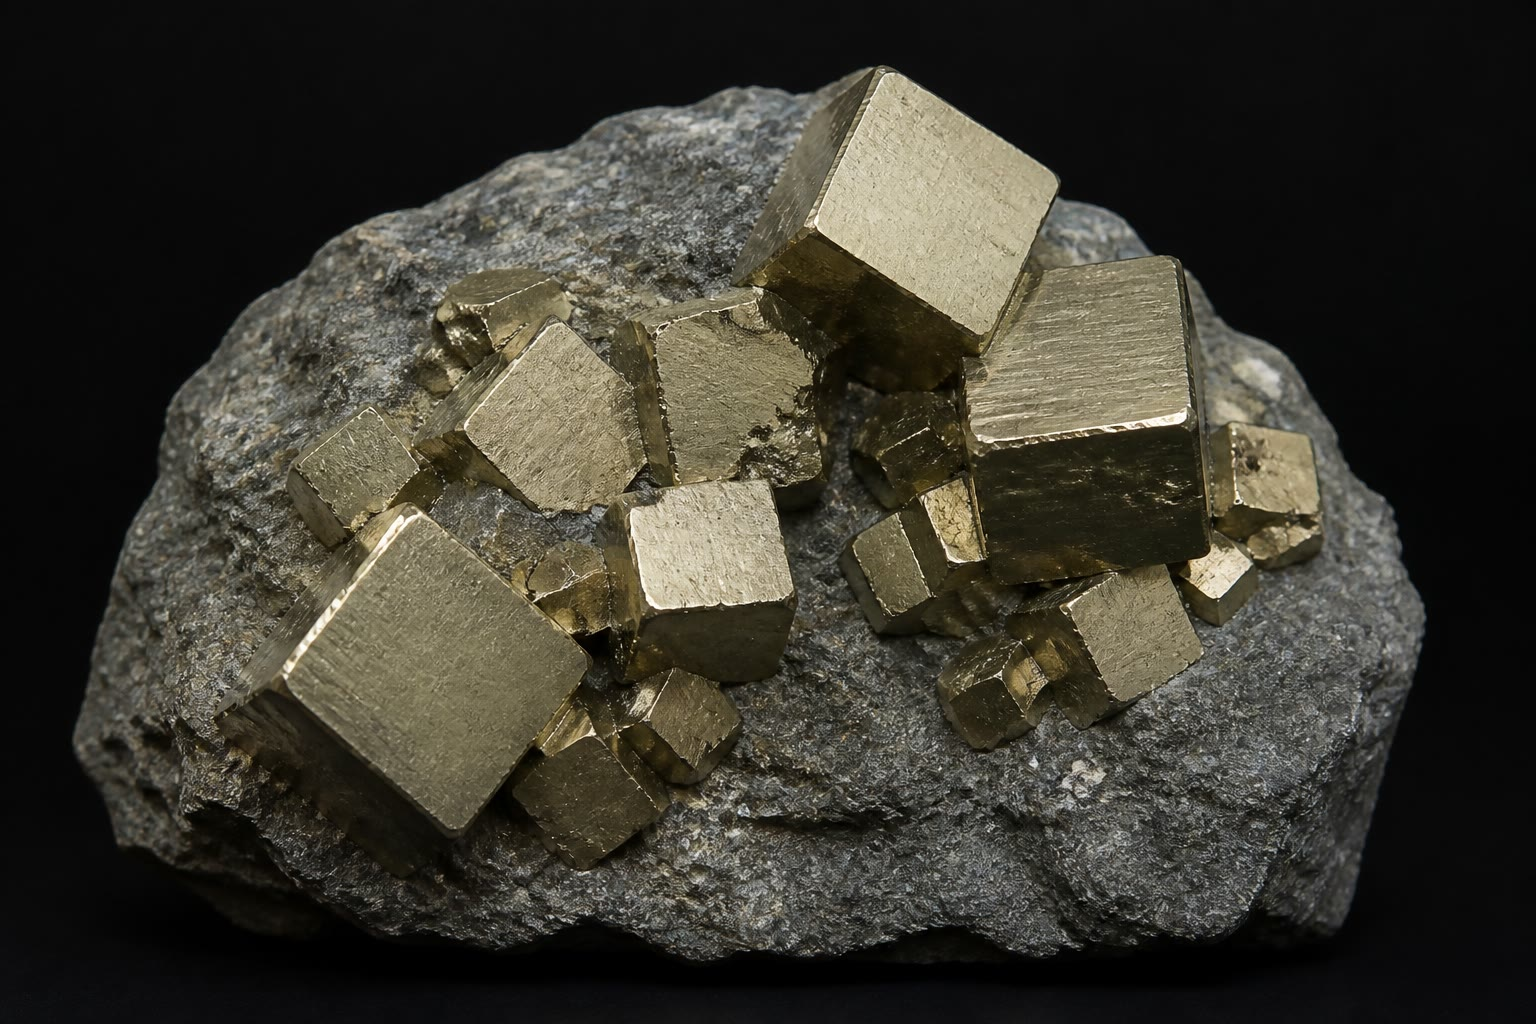
\includegraphics[width=0.58\linewidth]{images/book5/ai/b5-19-pyrite-cubes.jpg}

{\small 黄铁矿晶体：由地质作用生长而成的立方体，并非人工切割。其晶面为 (100) 晶面，原子有序排列，重复 $10^{23}$ 次，在人类尺度上显现。}
\end{omfigure}

\section{练习}

\begin{exercise}[$\star$]\label{exo:b3:crystalline-solids:1}
晶胞计数。（a）验证原子数：简单立方 1，体心立方 2，面心立方 4。
（b）在体心立方中，原子沿体对角线相接触，
用 $a$ 表示原子半径。（c）面心立方同理，原子沿
面对角线相接触。（d）计算堆积比
（$\pi\sqrt3/8 \approx 0.68$ 与 $\pi/\sqrt{18} \approx 0.74$），
并说明当成键无方向性时，金属
倾向于采用哪种结构。
\end{exercise}

\begin{exercise}[$\star$]\label{exo:b3:crystalline-solids:2}
铜的数值计算。面心立方，$a = \qty{3.61}{\angstrom}$，$M =
\qty{63.5}{g/mol}$。求（a）最近邻距离；
（b）最近邻数目；（c）密度；（d）
在 \qty{1}{\micro m} 的互连导线立方体中的原子数。
\end{exercise}

\begin{exercise}[$\star$]\label{exo:b3:crystalline-solids:3}
第一布拉格角。铜的 K$\alpha$ X 射线
（$\lambda = \qty{1.54}{\angstrom}$）射向间距为
$d = \qty{2.82}{\angstrom}$ 的 NaCl 晶面。（a）求一级角
$\theta_1$。（b）共有多少级？（c）为何任何反射都要求
$\lambda \le 2d$ 才能发生反射——又为何可见光
毫无希望？（d）若晶体受热，$\theta_1$ 将如何变化，
使 $d$ 膨胀 1\,\%？
\end{exercise}

\begin{exercise}[$\star$]\label{exo:b3:crystalline-solids:4}
晶面间距。对于晶格常数为 $a$ 的立方晶体：（a）将
晶面族 (100)、(110)、(111) 按间距排序，利用
$d = a/\sqrt{h^2+k^2+l^2}$。（b）哪一族在最小
布拉格角处发生反射？（c）金刚石沿
间距最大、结合最弱的晶面解理，是哪一族？（d）为何粉末样品
（大量随机取向的晶粒）会把布拉格斑点变为圆锥？
\end{exercise}

\begin{exercise}[$\star\star$]\label{exo:b3:crystalline-solids:5}
选择探针。（a）为何任何衍射探针都必须具有
$\lambda \sim \qty{1}{\angstrom}$？（b）X 射线光子的能量
是多少？（c）电子：利用本科二年级分册中
物质波的 $\lambda = h/p$，多大的加速电压可得到
\qty{0.05}{\angstrom}？（d）在 \qty{300}{K} 下的热中子：证明
$\lambda = h/\sqrt{3mk_{\text{B}}T} \approx \qty{1.5}{\angstrom}$，
并给出中子束能探测到 X 射线所遗漏结构的一个原因（提示：
X 射线被电子散射）。
\end{exercise}

\begin{exercise}[$\star\star$]\label{exo:b3:crystalline-solids:6}
用尺子数原子。NaCl：密度
$\rho = \qty{2165}{kg/m^3}$，摩尔质量 \qty{58.44}{g/mol}，
实测晶格常数 $a = \qty{5.64}{\angstrom}$（每个晶胞含 4 个 Na--Cl
对）。（a）写出 $\rho = 4M/N_{\text{A}}a^3$。（b）解出
$N_{\text{A}}$ 并求值。（c）考虑误差传递：
$a$ 中 0.1\,\% 的误差会使 $N_{\text{A}}$ 产生多大误差？（d）评注：
千克于 2019 年重新定义，部分借助这一晶体路线（
硅球）——为何该方法要求近乎完美的晶体？
\end{exercise}

\begin{exercise}[$\star\star$]\label{exo:b3:crystalline-solids:7}
马德隆账目。（a）对于无限长的 NaCl 交替电荷链，
间距为 $r_0$，证明每个离子的能量为
$-(e^2/4\pi\varepsilon_0r_0)\times2\ln2$——故一维
马德隆常数为 $2\ln2 \approx 1.386$。（b）
取 $\alpha = 1.7476$ 及 $r_0 = \qty{2.82}{\angstrom}$，求
$U$。（c）玻恩排斥项按 $r^{-9}$ 变化，最小化
$U(r) = -A/r + B/r^9$ 表明净束缚能为 $U(r_0)(1 - 1/9)$
——请重新估算。（d）与实测的每对
\qty{7.9}{eV} 相比较，并评论两项模型所得结果的意义。
\end{exercise}

\begin{exercise}[$\star\star$]\label{exo:b3:crystalline-solids:8}
伦纳德–琼斯氩。$\epsilon = \qty{0.0104}{eV}$，$\sigma =
\qty{3.40}{\angstrom}$。（a）求极小值点 $r_0 = 2^{1/6}
\sigma$，并与固态氩的实测值
\qty{3.76}{\angstrom} 相比较。（b）由
$k_{\text{B}}T_{\text{m}} \sim \epsilon/2$ 估算熔化温度，并与
\qty{84}{K} 相比较。（c）为何氦的质量极小、势阱很浅，
使其即便在绝对零度下仍保持液态（\cref{ch:b3:quantum-statistics}）？（d）
为什么范德瓦耳斯固体既柔软又易挥发，而金刚石
键能深三百倍，却能划伤一切？
\end{exercise}

\begin{exercise}[$\star\star$]\label{exo:b3:crystalline-solids:9}
由声音推知弹簧。（a）由
\cref{thm:b3:crystalline-solids:dispersion}，推出声速
$v = a\sqrt{K/m}$。（b）键弹簧近似为 $K \approx
Ea$，其中 $E$ 为杨氏模量，请用
拉伸晶胞的量纲分析加以论证。（c）对于铜（$E = \qty{1.2e11}{Pa}$，
$a = \qty{2.55}{\angstrom}$ 为原子间距，$m =
\qty{1.05e-25}{kg}$）：估算 $K$ 与 $v$，并与
实测值 $\sim\qty{4000}{m/s}$ 相比较。（d）为什么刚硬而轻的晶体
（金刚石）既具有最快的声速，又具有最高的
德拜温度？
\end{exercise}

\begin{exercise}[$\star\star\star$]\label{exo:b3:crystalline-solids:10}
布里渊区边界上的振动。（a）证明群速度
$\dd\omega/\dd k$ 在 $k = \pi/a$ 处为零。（b）写出原子
在该处的位移（$u_n \propto (-1)^n$），并描述其
运动。（c）解释：波长 $2a$ 满足
链本身的布拉格条件——该波即其自身的
衍射实验。（d）计算截止频率
$\omega_{\text{max}} = 2\sqrt{K/m}$，对
\cref{exo:b3:crystalline-solids:9}中的铜数据，并将其置于
电磁波谱的标度上。
\end{exercise}

\begin{exercise}[$\star\star\star$]\label{exo:b3:crystalline-solids:11}
每胞两个原子。在双原子链（质量 $m \ne M$）中，色散分裂为
\emph{声学支}（相邻原子同步运动：声音）与
\emph{光学支}（两个子晶格相互“拍击”），二者
之间隔着禁带。（a）为何在离子晶体中，光学模式
能否直接与
光耦合？（b）估算其在 NaCl 中的频率（$K \approx
\qty{25}{N/m}$，Na--Cl 对的约化质量）并求
对应波长。（c）由此解释为什么食盐在可见光中透明，
而在远红外中不透明（剩余射线）。（d）
为什么单原子链中不存在这样的禁带？
\end{exercise}

\begin{exercise}[$\star\star\star$]\label{exo:b3:crystalline-solids:12}
重建德拜模型。\cref{ch:b3:photons-phonons}中的德拜模型
仅保留 $\omega = vk$，并取截止波数以拟合模式数：
$k_{\text{D}} = (6\pi^2n)^{1/3}$。（a）论证模式数：
$N$ 个原子，共 $3N$ 个模式。（b）对于铜（$n = \qty{8.5e28}{m^{-3}}$，
平均声速 $v \approx \qty{2700}{m/s}$），计算
$k_{\text{D}}$ 与 $\Theta_{\text{D}} =
\hbar vk_{\text{D}}/k_{\text{B}}$，并与量热法测得的
\qty{343}{K} 相比较。（c）德拜的直线模型忽略了哪一种
真实色散特征（本章图中所示），并在哪些温度下这一差异
变得重要？（d）用一句话说明为何
$\Theta_{\text{D}}$ 与
\cref{exo:b3:crystalline-solids:10}中布里渊区边界处的截止频率是
同一物理在两种形式下的表现。
\end{exercise}

\section{周末问题：博物馆的锉屑}

\begin{problem}\label{pb:b3:crystalline-solids:1}
\emph{博物馆的锉屑。}一家海事博物馆回收了一块锈蚀的
取自十八世纪沉船的金属锭，并送给你们的实验室
几毫克锉屑：是贵金属，但究竟是哪一种？你们的粉末
衍射仪使用铜的 K$\alpha$ X 射线，
$\lambda = \qty{1.5406}{\angstrom}$。探测器通过扫描
偏转角 $2\theta$，在 $2\theta =
38.1^\circ$、$44.3^\circ$、$64.4^\circ$ 和 $77.5^\circ$ 处发现了强衍射环。

\medskip\noindent\textbf{第一部分——读取衍射环。}

\begin{enumerate}
  \item 叙述布拉格定律，并各用一句话说明
        单色光与粉末中随机取向的
        晶粒各自所起的作用。
  \item 将四个衍射环换算为 $\theta$，并
        计算每一个的 $\sin^2\theta$。
  \item 对于立方晶体，证明布拉格定律给出
        $\sin^2\theta = (\lambda^2/4a^2)(h^2 + k^2 + l^2)$。
  \item 将四个 $\sin^2\theta$ 值除以其中最小者：
        证明各比值接近 $1 : 1.33 : 2.67 : 3.67$，
        即 $3 : 4 : 8 : 11$ 除以 3。
  \item 面心立方晶体仅当 $h, k, l$ 全为偶数或
        全为奇数时才产生反射：检验 $(111)$、$(200)$、$(220)$、$(311)$——
        其和分别为 3、4、8、11——是否吻合，并说明缺失的和
        （1、2、5、6、7）能否借此区分面心立方与简单立方。
  \item 为什么体心立方金属（允许的和为 2、4、6、8、\dots）呈现
        不同的图样——以及为什么这种奇偶性判别，
        而非绝对角度，才是可靠的鉴定手段？
  \item 解释为什么晶粒长大后衍射环会变得更加锐利：一个
        五个原子宽的微晶对布拉格反射有何影响？
\end{enumerate}

\medskip\noindent\textbf{第二部分——确定金属种类。}

\begin{enumerate}[resume]
  \item 由每一个衍射环计算晶格常数 $a$，
        利用 $a = \lambda\sqrt{h^2+k^2+l^2}/2\sin\theta$。
  \item 对四个数值取平均，并将 $a$ 保留
        三位有效数字。
  \item 每个面心立方晶胞含 4 个原子，用
        $a$ 与摩尔质量 $M$ 表示密度。
  \item 可能的贵金属面心立方候选者：银
        （$M = \qty{107.9}{g/mol}$，$\rho = \qty{10.5}{g/cm^3}$）、
        金（$197.0$，$19.3$）、铂（$195.1$，$21.4$）。
        对每一种候选者，计算由你的 $a$ 所预言的密度，
        代入其 $M$，并判定金属锭的种类。
  \item 金的晶格常数为 $\qty{4.08}{\angstrom}$——
        与银几乎相同。本题中哪一个单独的测量
        仍能将二者区分开来？为什么它不受
        这一巧合影响？
  \item 博物馆要求对整个金属锭做无损检验。
        请提出一种方案（例如用阿基米德法测密度），并
        使其与你的微观结论相互印证。
\end{enumerate}

\medskip\noindent\textbf{第三部分——运动中的晶体。}

\begin{enumerate}[resume]
  \item 温热的银会振动：每个原子都在其格点附近晃动，
        均方位移 $\langle x^2\rangle \propto T$（键弹簧上的能量均分）。为什么这
        \emph{不会}使布拉格
        环变宽？
  \item 它确实会\emph{减弱}布拉格环：从偏离平衡位置的原子散射出的波
        失去同步性。请定性说明强度应如何随温度变化，
        即 $T$ 升高时的情形（德拜–沃勒
        效应）。
  \item 估算银的键弹簧：$K \approx Ea$，其中
        $E = \qty{8.3e10}{Pa}$，$a = \qty{2.89}{\angstrom}$
        为最近邻距离。
  \item 取 $m = \qty{1.79e-25}{kg}$，计算声速量级
        $v = a\sqrt{K/m}$，并与银的实测值
        $\sim\qty{2700}{m/s}$ 比较。
  \item 估算在 \qty{300}{K} 时的方均根热位移，
        由 $\tfrac12K\langle x^2\rangle \sim
        \tfrac32k_{\text{B}}T$ 可得，并将其与键长比较：
        该位移占键长的几分之几？
  \item 林德曼规则指出：当这一比值
        达到 $\sim10\,\%$ 时晶体熔化：请检验其与银
        在 \qty{1235}{K} 熔化这一事实是否相符。
\end{enumerate}

\medskip\noindent\textbf{第四部分——超越铸锭。}

\begin{enumerate}[resume]
  \item 铬是体心立方结构，$a = \qty{2.88}{\angstrom}$，预测
        其第一个环（(110) 族）的 $2\theta$，
        所用 X 射线与前述相同。
  \item 为什么电子显微镜能从表面和
        薄箔上产生衍射，而 X 射线和中子探测的是体材料？
        （用一句话说明每种粒子与物质的耦合强度。）
  \item 1952 年，一张拉伸纤维的衍射照片——
        呈 X 形排列的模糊斑点——揭示了沿螺旋堆叠的
        \qty{3.4}{\angstrom} 重复周期：这是哪种分子？
        为什么衍射能够成功，而显微镜
        却做不到？
  \item 铸造厂熔化了一块试样：请描述尖锐的
        环在液体的衍射图样中会变成什么，以及这说明
        液体保持着怎样的有序性。
  \item 准晶体给出具有五重对称性的尖锐斑点，这对任何
        周期性点阵都是不可能的。尽管如此，它的尖锐图样
        仍能证明其有序性的
        哪些方面？
  \item 用三句话总结这一判定：环的比值
        $\to$ 面心立方；$a = \qty{4.09}{\angstrom}$ $+$ 密度 $\to$
        银；以及晶体自身的振动 $\to$ 为何
        博物馆不应要求你对熔融态的晶体做 X 射线检测。
\end{enumerate}
\end{problem}
